V tejto kapitole sa oboznámime so základnými pojmami z bioinformatiky a
niektorými dátovými štruktúrami a algoritmami, ktoré budú neskôr použité pri
implementácii.

\section{Biologická motivácia}
\todo{}

\section{Formálne definície}

    \subsection{Zarovnanie}
    \begin{defn}
        Zarovnanie sekvencií $S_0 = a_1 a_2 \ldots a_n$ a $S_1 = b_1 b_2 \ldots
        b_m$ je funkcia $f : \mathbb{Z}_n \to \mathbb{Z}_m \cup \{ \bot \} $
        spĺňajúca nasledovnú podmienku:
        
        $ (\forall i, j \in \mathbb{Z}_n) (f(i) \neq \bot \wedge f(j) \neq \bot
        \wedge i < j) \implies (f(i) < f(j)) $
    \end{defn}
    
    \bigskip
    
    \begin{example}
        Dve možné zarovnania sekvencií $S_0$ = \texttt{AGGTA} a $S_1$ =
        \texttt{GCTA}:
        
        \bigskip
        
        \begin{minipage}{2.5in}
            \begin{tabular}{ c c c c c c c }
                0 & 1 & 2 &   & 3 & 4 \\ \hline     
                A & G & G & - & T & A \\
                - & G & - & C & T & A \\ \hline
                  & 0 &   & 1 & 2 & 3 \\   
            \end{tabular}
        \end{minipage}
        \begin{minipage}{2.5in}
            \begin{tabular}{ | c | c | }
                \hline            
                $i$ & $f(i)$ \\ \hline             
                0   & $\bot$ \\ \hline 
                1   & 0      \\ \hline
                2   & $\bot$ \\ \hline
                3   & 2      \\ \hline
                4   & 3      \\ \hline
            \end{tabular}
        \end{minipage}
        
        \bigskip
        
        \begin{minipage}{2.5in}
            \begin{tabular}{ c c c c c c c c c }
                0 & 1 & 2 & 3 & 4 &           \\ \hline     
                A & G & G & T & A & - & - & - \\
                - & - & G & - & - & C & T & A \\ \hline
                  &   & 0 &   &   & 1 & 2 & 3 \\   
            \end{tabular}
        \end{minipage}
        \begin{minipage}{2.5in}
            \begin{tabular}{ | c | c | }
                \hline            
                $i$ & $f(i)$ \\ \hline             
                0   & $\bot$ \\ \hline 
                1   & $\bot$ \\ \hline
                2   & 0      \\ \hline
                3   & $\bot$ \\ \hline
                4   & $\bot$ \\ \hline
            \end{tabular}
        \end{minipage}        
    \end{example}
    
\bigskip
    
\todo{chcem viac o zarovnavaniach ? globalne zarovnanie, skorovanie atd}

\section{Definícia problému}

Úlohou bude vytvoriť efektívnu dátovú štruktúru, ktorá načíta veľkú sadu
relatívne krátkych \emph{sequence reads} a umožní v nich rýchlo vyhľadávať.
Počty týchto \emph{readov} sa budú pohybovať v miliónoch až desiatkach miliónov
a ich dĺžka bude 100-500 báz. 

Konkrétnejšie, budeme požadovať, aby táto štruktúra spĺňala nadsledovné
podmienky:

\begin{itemize}
    \item načíta sadu reťazcov (\emph{sequence reads}), ktoré pochádzajú z
    jedného spoločného nadslova (genómu, ktorý bol sekvenovaný). Treba rátať s
    chybami pri sekvenovaní, t.j. jednotlivé načítavané reťazce môžu mať jemné
    odlišnosti oproti spoločnému nadslovu.
    \item bude sa v nej dať vyhľadávať podľa viacerých kritérií (časom uvidíme,
    aké konkétne to budú), napr. ``obsahuje podreťazec $P$''.
    \item bude mat čo najmenšiu pamätovú zložitost, pri zachovaní rozumnej
    časovej, cieľom by malo byť niečo typu $O(n + s)$, kde $n$ je počet
    načítaných reťazcov a $s$ je dĺžka spoločného nadslova. (Triviálnym riešením
    by bolo $O(nl)$, kde $l$ je dĺžka readu).
\end{itemize}

\newpage % TODO: remove this

\section{Related work}
\todo{spomenut bezne rieseny, no opacny problem - zarovnavanie  genomu - tam sa
indexuje referencny genom v nejakej super efektivnej DS, sequence ready sa potom
paralelne spracuvaju ako sa citaju. my chceme mat efektivne zaindexovane velke
mnozstvo readov, aby sme to vedeli kadejako efektivne filtrovat }



\section{Funkcie rank a select}
\begin{defn}
    Funkcia $rank$ na reťazci $S$ je definovaná ako $rank_S(i, c) = n$, kde $n$
    predstavuje počet výskytov znaku $c$ v reťazci $S[1, i]$. Ak $i \leq 0$,
    potom $rank_S(i, c) = 0$.
\end{defn}

\begin{defn}
    Funkcia $select$ na reťazci $S$ je definovaná ako $select_S(n, c) = i$, kde
    $i$ predstavuje najmenší index v reťazci $S$, pre ktorý platí, že počet
    výskytov znaku $c$ v $S[1, i]$ je $n$. Funkcia $select$ je inverzná funkcia
    ku funkcii $rank$.
\end{defn}

\begin{example}
    $S = banana$. Potom $rank_S(4, a) = 2$ a $select_S(1, n) = 3$.
\end{example}

\todo{pokec o zlozitosti jednotlivych implementacii rank a select?}

\section{Sufixové polia}

Sufixové pole je jednoduchá dátová štruktúra používaná napríklad pri indexácii,
kompresných algoritmoch alebo v bioinformatike. Tento koncept bol predstavený v
roku 1990 \cite{MM90}. Bol navrhnutý ako pamäťovo efektívnejšia náhrada
sufixových stromov.

\begin{defn}
    Nech $S = s_1 s_2 \ldots s_n$ je reťazec a nech $S[i, j]$ označuje
    podreťazec reťazca $S$ od $i$ po $j$, t.j. $s_i s_{i+1} \ldots s_{j-1} s_j$.
    Sufixové pole $SA$ reťazca $S$ je pole kladných čísel označujúcich začiatočné pozície sufixov reťazca $S$ v
    lexikografickom usporiadaní.
\end{defn}

K reťazcom sa zvykne na konci pridávať špeciálny znak \$, ktorý sa v
lexikografickom usporiadaní nachádza pred všetkými znakmi uvažovanej abecedy.

\begin{example}
    Nech $S = banana\$$. Usporiadané sufixy $S$ budú vyzerať nasledovne:
    \begin{center}
        \begin{tabular}{ | l | l | }
            \hline
            \textbf{sufix} & \textbf{i} \\ \hline
            \$             & 7          \\ \hline
            a\$            & 6          \\ \hline
            ana\$          & 4          \\ \hline
            anana\$        & 2          \\ \hline
            banana\$       & 1          \\ \hline
            na\$           & 5          \\ \hline
            nana\$         & 3          \\ \hline
        \end{tabular}
    \end{center}
    
    Prislúchajúce sufixové pole: $SA = (7, 6, 4, 2, 1, 5, 3)$.
\end{example}

    \subsection{Vyhľadávanie vzorky v sufixovom poli}
    Vyhľadávanie všetkých výskytov vzorky $P$ v texte $S$ vlastne znamená nájsť
    všetky sufixy $S$, ktoré začínajú na $P$, t.j. hľadáme taký úsek od $i$ po
    $j$ v sufixovom poli $SA$, pre ktorý platí, že
    $\forall k: i \leq k \leq j: S[SA[k], \lvert S \rvert] = P$. Kedže je
    sufixové pole usporiadané, môžeme použiť binárne vyhľadávanie. V tomto
    prípade bude zložitosť algoritmu $O(\lvert P \rvert \log \lvert S \rvert)$.
    (Porovnanie dvoch reťazcov dľžky $n$ je realizované v čase $O(n)$). Použitím
    $LCP$ (least common prefix) je možné tento čas vylepšiť na $O(\lvert P
    \rvert + \log{\lvert S \rvert})$. Idea spočíva v tom, že pri porovnávaní
    reťazcov nie je potrebné niektoré znaky porovnávať znovu, ak vieme, že sú
    súčasťou $LCP$ - najdlhšieho spoločného prefixu - vzorky a momentálneho
    prehľadávaného intervalu. V roku 2004 bol predstavený algoritmus
    \cite{AKO04} pracujúci v čase dokonca $O(\lvert P \rvert)$.
    
    \subsection{Konštrukcia sufixového poľa}
    \begin{description}
        \item[Klasické triedenie]        \hfill \\
        Merge sort potrebuje $O(n \log{n})$ porovnaní, no porovnanie každej
        dvojice sufixov trvá $O(n)$, takže dokopy konštrukcia sufixového poľa
        potrvá $O(n^2 \log{n})$.
        \item[Radix sort]                \hfill \\
        Triedenie pomocou radix sortu predstavuje mierne zlepšenie. Radix sort
        vo všeobecnosti triedi $d$ ciferné čísla v $k$-árnej sústave, pričom
        každú cifru triedi pomocou counting sortu. Ten utriedi $n$ čísel z
        množiny ${0 \ldots k - 1}$ v čase $O(n + k)$. Celkový čas radix sortu je
        teda $O(d (n + k))$. Ak uvažujeme abecedu ako podmnožinu množiny ${0,
        \ldots, n - 1}$, tak nám čas triedenia vyjde $O(n^2)$.
        \item[Pomocou sufixového stromu] \hfill \\
        Ak najprv skonštruujeme sufixový strom (to sa dá spraviť v čase $O(n)$)
        a potom ho postupne prechádzame do hĺbky, pričom v každom vrchole
        prechádzame neprejdené hrany podľa abecedy, tak potom poradie, v ktorom
        navštívime listy predstavuje poradie sufixov v sufixovom poli.
        Nepríjemnosťou pri tomto postupe je fakt, že sufixové stromy zaberajú
        príliš veľa pamäte.
        \item[Lineárne algoritmy]        \hfill \\
        Lineárnych algoritmov existuje niekoľko, napríklad \emph{SA-SI}
        \cite{NZC09}, ktorý je momentálne jeden z najrýchlejších známych
        algoritmov, prípadne algoritmus od Kärkkäinena a Sandersa \cite{KS03}.
        
        \todo{chcem tu nejak velmi rozpisovat nejaky konkretny linearny algoritmus?}
    \end{description}
    
    \subsection{Pamäťová efektivita}
    Sufixové polia sú vo všeobecnsti efektívnejšie než sufixové stromy, no v
    niektorých prípadoch to nestačí. Sufixové pole vyžaduje $O(n \log{n})$
    bitov, kdežto pôvodný text nad abecedou $\sigma$ len $O(n
    \log{\lvert \sigma \rvert})$. Pre ľudský genóm ($\sigma = \{A, C, T, G\}, n
    = 3.4 \times 10^9$) by teda sufixové pole zaberalo približne 16 krát viac
    pamäte než samotný genóm. Práve z tohto dôvodu sa objavili vylepšenia ako
    napríklad \textit{komprimované sufixové polia} a \textit{FM-index}.
    
    \todo{rozpisat rozpisat vypocet hodnot LCP pre sufixove pole (?)}

\section{Burrows-Wheelerova transformácia}
    Burrows-Wheelerova transformácia (BWT) je transformácia textu využívaná pri
    kompresii (napríklad v programe bzip2) ale aj v úsporných dátových
    štruktúrach na hľadanie vzorky v texte. BWT transformuje vstupný reťazec $S$
    na reťazec $bw(S)$, ktorý je permutáciou pôvodného reťazca, no s tou
    vlastnosťou, že sa dá väčšinou oveľa lepšie skomprimovať než pôvodný
    reťazec. Táto transformácia je invertovateľná (bez potreby uloženia
    akýchkoľvek dát navyše), t.j. z reťazca $bw(S)$ vieme získať pôvodný reťazec
    $S$.
    
    \subsection{BWT cez BWM}
    \subsubsection*{Postup transformácie}
    \begin{itemize}
        \item na koniec reťazca $S$ pridáme špeciálny symbol \$, ktorý sa
        nevyskytuje v danej abecede a zadefinujeme ho ako prvý symbol novej
        abecedy (vzhľadom na lexikografické usporiadanie)
        \item vytvoríme maticu cyklických posunov reťazca $S\$$
        \item lexikograficky utriedime riadky matice
        \item posledný stĺpec matice predstavuje $bw(S)$
    \end{itemize}
    
    Táto lexikograficky utriedená matica cyklických posunov reťazca $S$
    sa označuje ako BWM (Burrows-Wheeler matrix).
    
    \begin{example}
        Uvažujme $S = banana\$$. Matica cyklických posunov a utriedená matica 
        budú vyzerať nasledovne:
        
        \bigskip
        
        \begin{minipage}{2.5in}
            \begin{tabular}{ c c c c c c c }
                b  & a  & n  & a  & n  & a  & \$ \\
                a  & n  & a  & n  & a  & \$ & b  \\
                n  & a  & n  & a  & \$ & b  & a  \\
                a  & n  & a  & \$ & b  & a  & n  \\
                n  & a  & \$ & b  & a  & n  & a  \\
                a  & \$ & b  & a  & n  & a  & n  \\
                \$ & b  & a  & n  & a  & n  & a  \\
            \end{tabular}
        \end{minipage}
        \begin{minipage}{2.5in}
            \begin{tabular}{ c c c c c c c }
                \$ & b  & a  & n  & a  & n  & \textbf{a}  \\            
                a  & \$ & b  & a  & n  & a  & \textbf{n}  \\
                a  & n  & a  & \$ & b  & a  & \textbf{n}  \\
                a  & n  & a  & n  & a  & \$ & \textbf{b}  \\
                b  & a  & n  & a  & n  & a  & \textbf{\$} \\
                n  & a  & \$ & b  & a  & n  & \textbf{a}  \\ 
                n  & a  & n  & a  & \$ & b  & \textbf{a}  \\
            \end{tabular}
        \end{minipage}
        
        \bigskip
        
        Teda $bw(banana\$) = annb\$aa$ - posledný stĺpec utriedenej matice.
    \end{example}

    \subsection{BWT cez sufixové pole}
    Medzi BWM a sufixovým poľom je zjavný súvis - pri vytváraní sufixového poľa
    $SA(S)$ pre reťazec $S$ triedime sufixy reťazca $S$ a pri vytváraní $BWM(S)$
    triedime cyklické posuny $S$. Tento vzťah je jasnejší v príklade:
    
    \bigskip
    
    \begin{example}
        \begin{tabular}{ | l  | r | l | }
            \hline
            \textbf{BWM} & \textbf{SA} & \textbf{sufix $S$} \\ \hline 
            \$banana     & 7           & \$                 \\ \hline
            a\$banan     & 6           & a\$                \\ \hline
            ana\$ban     & 4           & ana\$              \\ \hline
            anana\$b     & 2           & anana\$            \\ \hline
            banana\$     & 1           & banana\$           \\ \hline
            na\$bana     & 5           & na\$               \\ \hline
            nana\$ba     & 3           & nana\$             \\ \hline
        \end{tabular}
    \end{example}
    
    \bigskip
    
    Iný spôsob ako definovať $BWT(S)$ je teda cez sufixové pole $SA(S)$:
    
    \bigskip
    
    $
        BWT(S)[i] = \begin{cases}
                        S[SA[i]] & : SA[i] > 1 \\ 
                        \$       & : SA[i] = 1
                    \end{cases}
    $                    
    
    \subsection{Reverzná BTW s použitím LF mappingu}
    Na začiatku teda poznáme len $BWT(S)$, čo je posledný stĺpec (označme ho
    $L$) matice lexikograficky usporiadaných cyklických rotácií povôdného
    reťazca $S$. Z neho si vieme spočitať prvý stĺpec ($F$) matice jednoduchým
    utriedením posledného stĺpca:
    
    \bigskip
    
    \begin{example}
        \begin{tabular}{ c c c }
            \textbf{F}   &        & \textbf{L} \\  
            \$           & \ldots & a          \\
            a            & \ldots & n          \\
            a            & \ldots & n          \\
            a            & \ldots & b          \\
            b            & \ldots & \$         \\
            n            & \ldots & a          \\
            n            & \ldots & a          \\
        \end{tabular}
    \end{example}
    
    \bigskip    
    
    Pripomeňme si ešte pôvodnú, kompletnú maticu s tým, že každému znaku
    pridáme ako dolný index jeho $rank_S$ vzhľadom na pôvodný reťazec $S$ (kde
    ako $i$ dosadíme jeho index v $S$). Môžme si všimnúť, že relatívne
    poradie písmen je v $L$ a $F$ rovnaké.
    
    \bigskip
    \begin{example}
        \begin{tabular}{ c c c c c c c }
            \textbf{F}         &
                               &
                               &
                               &
                               &
                               &
            \textbf{L}         \\
        
            \$                 &
            b\textsubscript{1} &
            a\textsubscript{1} &
            n\textsubscript{1} &
            a\textsubscript{2} & 
            n\textsubscript{2} &
            a\textsubscript{3} \\
            
            a\textsubscript{3} &
            \$                 &
            b\textsubscript{1} &
            a\textsubscript{1} &
            n\textsubscript{1} &
            a\textsubscript{2} & 
            n\textsubscript{2} \\
            
            a\textsubscript{2} &
            n\textsubscript{2} &
            a\textsubscript{3} &
            \$                 &
            b\textsubscript{1} &
            a\textsubscript{1} &
            n\textsubscript{1} \\
            
            a\textsubscript{1} &
            n\textsubscript{1} &
            a\textsubscript{2} &
            n\textsubscript{2} &
            a\textsubscript{3} &
            \$                 &
            b\textsubscript{1} \\
            
            b\textsubscript{1} &
            a\textsubscript{1} &
            n\textsubscript{1} &
            a\textsubscript{2} &
            n\textsubscript{2} &
            a\textsubscript{3} &
            \$                 \\
            
            n\textsubscript{2} &
            a\textsubscript{3} &
            \$                 &
            b\textsubscript{1} &
            a\textsubscript{1} &
            n\textsubscript{1} &
            a\textsubscript{2} \\ 
            
            n\textsubscript{1} &
            a\textsubscript{2} &
            n\textsubscript{2} &
            a\textsubscript{3} &
            \$                 &
            b\textsubscript{1} &
            a\textsubscript{1} \\
        \end{tabular}
    \end{example}
    \bigskip
    
    Ďalej platí, že $F[i]$ nasleduje po $L[i]$ v $S$. Preto v našom príklade
    symbolu \$ v $L$ prislúcha $S[0] = b$. Potom nájdeme $S[0]$ v $L$, dostaneme
    $S[1]$ v $F$ ($S[1] =$ tretie $a$). Nájdeme tretie $a$ v $L$, dostaneme
    $S[2]$ v $F$ ($S[2] =$ druhé $n$) atď.
    
    Je nutné ale poznamenať, že problémom môže byť, ak je pôvodný reťazec $S$
    veľmi dlhý - vtedy je neefektívne prepočítať si $rank$ pre všetky znaky,
    nakoľko by táto informácia zaberala oveľa viac pamäte než $BWT(S)$. Preto je
    táto inverzná operácia v praxi riešená inak. 

    \todo{pohladat, ako je to
    riesene. okrem toho, ze bzip2 to vraj komprimuje 'into relatively small
    blocks, decompressing a block at time'}
    
\section{FM index}  
    \todo{} % TODO

    \subsection{Vyhľadávanie pomocou FM indexu}
    \todo{} % TODO
    
    \subsection{Zlepšenia - offsets, rrank checkpoints}
    \todo{} % TODO
    
\section{Algoritmy na zostavovanie genómu}
    Výsledkom sekvenovania genómu (pri použití súčasných technológií) je veľké
    množstvo malých fragmentov - \emph{sequencing reads}, ktoré je potrebné
    zostaviť do jednej súvislej sekvencie. Náročnosť tejto úlohy závisí najmä
    od:
    
    \begin{itemize}
        \item dĺžky zostavovaného genómu - čím je kratší, tým je to jednoduchšie
        \item dĺžok jednotlivých fragmentov - čím sú dlhšie, tým lepsie
        \item priemernej hĺbky pokrytia - tzn koľko fragmentov v priemere
        pokrýva konkrétnu pozíciu zostavovanej sekvencie - čím viac, tým lepšie
    \end{itemize}

    \subsection{Najkratšie spoločné nadslovo}
    Asi najjednodušiu formuláciu problému zostavovania genómu predstavuje
    problém hľadania najkratšieho spoločného nadslova (\emph{shortest common
    superstring}).
    
    \begin{defn}
        Najkratším spoločným nadslovom reťazcov $S_1, S_2, \ldots, S_k$ nazývame
        najkratší reťazec $S$ taký, že každé $S_i$ je podslovo $S$.
    \end{defn}
    
    Tento problém je ale NP-ťažký, takže nepoznáme žiadny rýchly algoritmus,
    ktorý vždy nájde riešenie. Jednoduchá heuristika by vyzerala nasledovne:
    
    \begin{itemize}
        \item nájdi také dva fragmenty, ktoré majú najväčší prekryv, t.j.
        najdlhšiu $\alpha$ takú, že $S_i = \alpha\beta$ a $S_j = \gamma\alpha$
        \item spoj $S_i$ a $S_j$ do $\gamma\alpha\beta$
        \item opakuj prvý krok, kým neozostane iba jedno slovo
    \end{itemize}
    
    O tomto algorime sa dá dokázať, že je to 3.5-aproximačný algoritmus, t.j.
    nájdené riešenie bude mať vždy dĺžku nanajvýš 3.5-násobku optimálnej dĺžky.
    Síce je problém najkratšieho spoločného nadslova pomerne elegantnou
    formuláciou problému zostavovania genómov, je tento problém príliš ťažký na
    to, aby bolo jeho riešenie praktické pre veľké genómy. Preto sa v praxi
    používajú iné metódy.

    \subsection{Overlap-Layout-Consensus}
    Táto metóda, ako už jej názov naznačuje, pracuje v troch fázach:
    
    \begin{description}
        \item[Overlap]        \hfill \\
        V tejto fáze assembler hľadá navzájom sa prekrývajúce fragmenty a spája
        ich do dlhších fragmentov, \emph{kontigov}.
        
        Porovnávanie každej dvojice fragmentov by však bolo v praxi veľmi časovo
        náročné, nakoľko fragmentov môžu byť často milióny a pri porovnaní
        každej dvojice by sme potrebovali rádovo $O(n^2k)$ času (kde $n$ je
        počet fragmentov a $O(k)$ je čas, ktorý trvá porovnanie dvoch
        fragmentov).
        
        Efektívnejšie algoritmy sú založené na predpoklade, že ak sa dva
        fragmenty úplne zhodujú na úseku dľžky aspoň $k$ (v praxi sa používa $k
        \approx 24$ ), tak pochádzajú z toho istého miesta v sekvenovanom genóme
        a teda sú spojené do jedného kontigu.
        
        Vo všeobecnosti vyzerá tento postup nasledovne:
        \begin{itemize}
            \item vytvor zoznam podreťazcov dĺžky $k$ zo všetkých fragmentov,
            pričom ku každému podreťazcu si zapamätaj, z ktorého fragmentu
            pochádza
            \item lexikograficky utrieď zoznam podreťazcov
            \item skupiny výrazne sa prekrývajúcich fragmentov sa v utriedenom
            zozname budú vyskytovať pohromade a práve to sú dobrí kandidáti na
            spojenie do kontigov
        \end{itemize}
        \item[Layout] \hfill \\
        V druhej fáze assembler určuje relatívnu polohu jednotlivých kontigov a
        ich približné vzdialenosti, výsledné bloky kontigov sa nazývajú
        \emph{superkontigy}.
        \item[Consensus] \hfill \\
        V poslednej fáze je vytvorená finálna sekvencia superkontigov, ktorá
        pokrýva genóm (alebo aspoň jeho časti).
    \end{description}
    
    Často sa ale zvykne používať aj grafová reprezentácia tohto algoritmu.
    Vrcholmi grafu sú fragmenty, hrana medzi vrcholmi je vtedy, ak sa tieto dva
    fragmenty prekrývajú (overlap). V layout fáze sa tento graf zjednodušuje
    (napr. vymazanie nadbytočných hrán). Fáza consensus potom spočíva v nájdení
    hamiltonovskej cesty v tomto grafe.
    
    \subsection{De Bruijnove grafy}
    Tento prístup využíva to, že (obvykle) máme pri sekvenovaní veľké množstvo
    dát, a preto si môžme dovoliť časť obsiahnutej informácie v nich
    odignorovať.
    
    Pre jednoduchosť budeme predpokladať, že všetky fragmenty pochádzajú z
    jedného vlákna a snažíme sa zostaviť len jeden, úplne pokrytý chromozóm.

    Algoritmus pre vytvorenie \emph{de Bruijnovho grafu} vyzerá nasledovne:
    
    \begin{itemize}
        \item vytvor zoznam všetkých podreťazcov dĺžky $k$ zo všetkých
        fragmentov ($k$-tice)
        \item vrcholy grafu budú tvoriť všetky úseky dĺžky $k - 1$ (teda
        podreťazce podreťazcov dĺžky $k$)
        \item jednotlivé $k$-tice budú reprezentované orientovanými hranami v
        grafe, pričom $k$-tica $s_1 s_2 \ldots s_k$ spája vrcholy $s_1 s_2
        \ldots s_{k-1}$ a $s_2 s_3 \ldots s_k$. 
    \end{itemize}
    
    Eulerovský ťah v takomto grafe potom predstavuje hľadaný genóm.
    
    \begin{example}
        Uvažujme fragmenty \texttt{CCTGCC} a \texttt{GCCACC} a $k = 3$. Zoznam
        $k$-tic teda bude vyzerať nasledovne:
        
        \bigskip
        
        \begin{tabular}{ c c }
            \textbf{CCTGCC} & \textbf{GCCACC} \\  
            \texttt{CCT}    & \texttt{GCC}    \\
            \texttt{CTG}    & \texttt{CCA}    \\
            \texttt{TGC}    & \texttt{CAC}    \\
            \texttt{GCC}    & \texttt{ACC}    \\
        \end{tabular}  
        
        \bigskip
        
        Úseky dĺžky $k-1$: \texttt{CC}, \texttt{CT}, \texttt{TG}, \texttt{GC},
        \texttt{CA}, \texttt{AA}, \texttt{AC}
        
        \bigskip
        
        Graf: 
        
        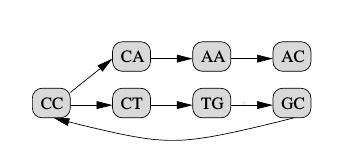
\includegraphics{graf.png}
    \end{example}